
\section{Experimento BRDF Blinn-Phong} \label{section-experiment-blinn-phong}

Neste experimento usamos uma BRDF com um método simplificado de cálculo de reflexão especular, presente na \autoref{fig-blinn-phong-eqlang-latex}, introduzido por Blinn-Phong \cite{blinn1977models}. O \autoref{cod-blinn-phong-eqlang}, escrito \texttt{EquationLang}, é a entrada para o compilador. O \autoref{cod-blinn-phong-glsl-pt-1} e \autoref{cod-blinn-phong-glsl-pt-2} são a sáida em GLSL. A renderização dos objetos 3D estão na \autoref{fig-blinn-phong-eqlang}. Por fim, os \textit{plots} estão na \autoref{fig-blinn-phong-plots}.

%%%%%%%%%%%%%%%%%%%%%%%%%%%%%%%%%%%%%%%%%%%%%%%%%
\subsection{Representação em documento \LaTeX{}}
%%%%%%%%%%%%%%%%%%%%%%%%%%%%%%%%%%%%%%%%%%%%%%%%%
\begin{figure}[H]
    \caption{\label{fig-blinn-phong-eqlang-latex} 
    \small Equações da BRDF do experimento Blinn-Phong em documento \LaTeX{}.}
    \begin{center}
        % 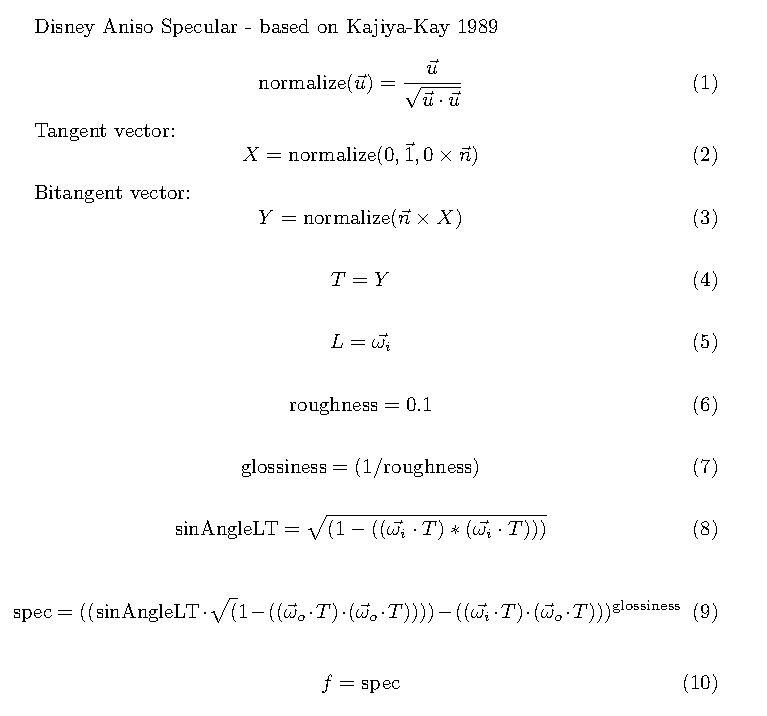
\includegraphics[scale=1.1,width=\textwidth]{./Imagens/brdfs/aniso.pdf}
        
\includegraphics[scale=0.92]{./Imagens/brdfs/blinn-phong.pdf}
    \end{center}
\end{figure}


%%%%%%%%%%%%%%%%%%%%%%%%%%%%%%%%%%%%%%%%%%%%%%%%%
\subsection{Código Fonte em \texttt{EquationLang}}
%%%%%%%%%%%%%%%%%%%%%%%%%%%%%%%%%%%%%%%%%%%%%%%%%
\begin{codigo}[H]
    \caption{\small Código fonte da BRDF do experimento Blinn-Phong.}
    \label{cod-blinn-phong-eqlang}
\begin{lstlisting}[language=tex, frame=none, inputencoding=utf8]
\begin{equation}
    \rho_{d} = \vec{0,1,1}
\end{equation}

\begin{equation}
    \rho_{s} = \vec{1,0,1}
\end{equation}

\begin{equation}
    n = +2^8
\end{equation}

\begin{equation}
f = \frac{\rho_{d}}{\pi} + \rho_{s} * \frac{n+2}{2*\pi} *
\cos{\theta_{h}}^{n}
\end{equation}
\end{lstlisting}
\end{codigo}

%%%%%%%%%%%%%%%%%%%%%%%%%%%%%%%%%%%%%%%%%%%%%%%%%
\subsection{Código GLSL Gerado}
%%%%%%%%%%%%%%%%%%%%%%%%%%%%%%%%%%%%%%%%%%%%%%%%%
\begin{codigo}[H]
    \caption{\small Saída do compilador: código GLSL da BRDF do experimento Blinn-Phong (parte 1 de 2).}
    \label{cod-blinn-phong-glsl-pt-1}
\begin{lstlisting}[language=C, inputencoding=utf8]
analytic ::begin parameters
#[type][name][min val][max val][default val]
::end parameters
::begin shader
//////////// START OF BUILTINS DECLARTION ////////////
vec3 var_0_vec_h;
vec3 var_3_vec_n;
float var_10_theta_h;
float var_11_theta_d;
float var_1_pi;
float var_2_epsilon;
vec3 var_4_vec_omega_i;
float var_5_theta_i;
float var_6_phi_i;
vec3 var_7_vec_omega_o;
float var_8_theta_o;
float var_9_phi_o;
//////////// END OF BUILTINS DECLARTION ////////////
//////////// START OF USER DECLARED ////////////
vec3 var_12_rho_s;
float var_13_n;
vec3 var_14_rho_d;
vec3 var_15_f;
//////////// END OF USER DECLARED ////////////
\end{lstlisting}
\end{codigo}

\begin{codigo}[H]
    \caption{\small Saída do compilador: código GLSL da BRDF do experimento Blinn-Phong (parte 2 de 2).}
    \label{cod-blinn-phong-glsl-pt-2}
\begin{lstlisting}[language=C, inputencoding=utf8]
vec3 BRDF(vec3 L, vec3 V, vec3 N, vec3 X, vec3 Y) {
  //////////// START OF BUILTINS INITIALIZATION ////////////
  var_0_vec_h = normalize(L + V);
  var_3_vec_n = normalize(N);
  var_1_pi = 3.141592653589793;
  var_2_epsilon = 1.192092896e-07;
  var_4_vec_omega_i = L;
  var_5_theta_i = atan(var_4_vec_omega_i.y, var_4_vec_omega_i.x);
  var_6_phi_i = atan(sqrt(var_4_vec_omega_i.y * var_4_vec_omega_i.y +
                          var_4_vec_omega_i.x * var_4_vec_omega_i.x),
                     var_4_vec_omega_i.z);
  var_7_vec_omega_o = V;
  var_8_theta_o = atan(var_7_vec_omega_o.y, var_7_vec_omega_o.x);
  var_9_phi_o = atan(sqrt(var_7_vec_omega_o.y * var_7_vec_omega_o.y +
                          var_7_vec_omega_o.x * var_7_vec_omega_o.x),
                     var_7_vec_omega_o.z);
  var_10_theta_h = acos(dot(var_0_vec_h, N));
  var_11_theta_d = acos(dot(var_0_vec_h, var_4_vec_omega_i));
  //////////// END OF BUILTINS INITIALIZATION ////////////
  var_12_rho_s = vec3(1.0, 0.0, 1.0);
  var_13_n = pow(2.0, 8.0);
  var_14_rho_d = vec3(0.0, 1.0, 1.0);
  var_15_f = ((var_14_rho_d / var_1_pi) +
              ((var_12_rho_s * ((var_13_n + 2.0) / (2.0 * var_1_pi))) *
               pow(cos(var_10_theta_h), var_13_n)));

  return vec3(var_15_f);
}
\end{lstlisting}
\end{codigo}

%%%%%%%%%%%%%%%%%%%%%%%%%%%%%%%%%%%%%%%%%%%%%%%%%
\subsection{Visualização do Resultado}
%%%%%%%%%%%%%%%%%%%%%%%%%%%%%%%%%%%%%%%%%%%%%%%%%

\begin{figure}[H]
  
    \caption{\small{\textit{Plots} da distribuição de reflexão especular e difusa do experimento Blinn-Phong.}}
    \label{fig-blinn-phong-plots}
\minipage{0.48\textwidth}
    \vspace{42px}
  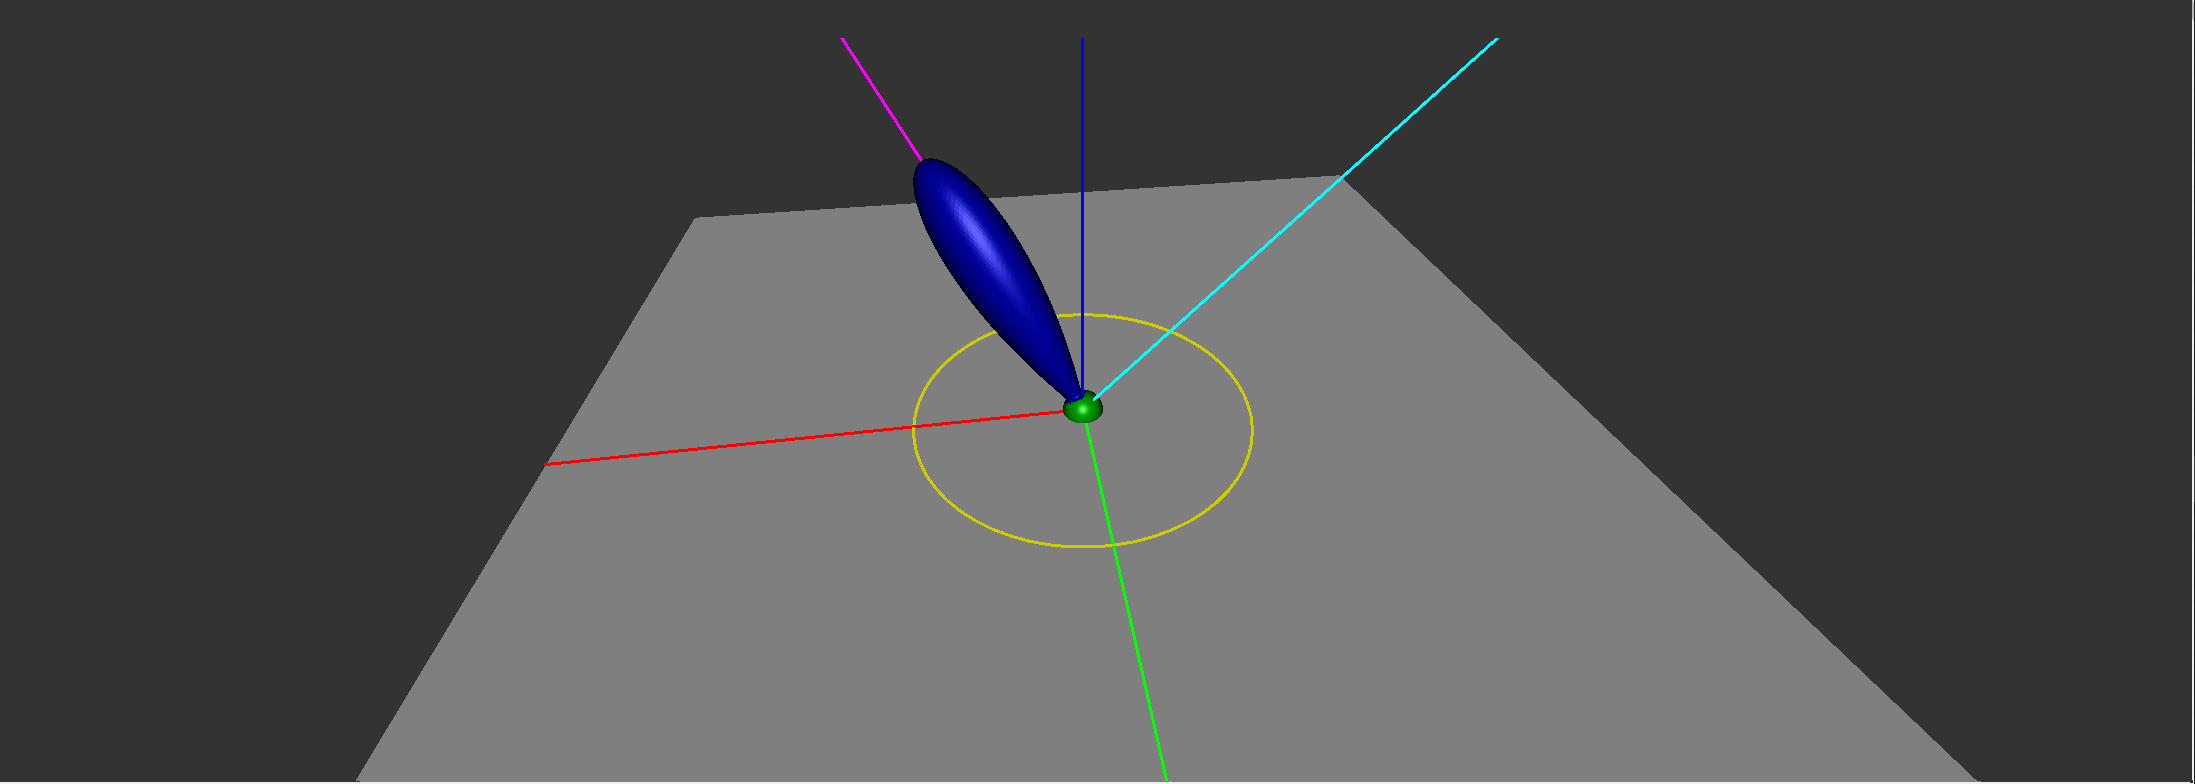
\includegraphics[width=\linewidth]{./Imagens/brdfs/blinn-phong-3D-plot}
    % \caption{\small{(a)}}\label{fig:awesome_image1}
    % \vspace{0.1px}
    \legend{ \small (a) 3D \textit{plot}}
\endminipage\hfill
\minipage{0.48\textwidth}
  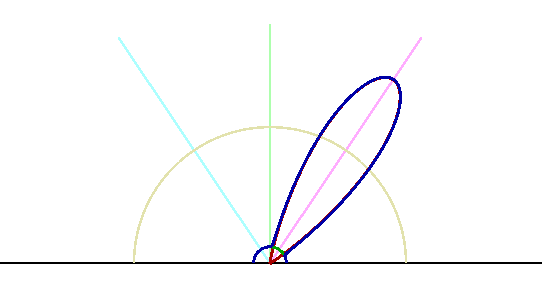
\includegraphics[width=\linewidth]{./Imagens/brdfs/blinn-phong-polar-plot-log.png}
    \legend{ \small (b) \textit{Polar plot}}
    % \caption{\small{(b)}}\label{fig:awesome_image1}
\endminipage\hfill
\end{figure}

\begin{figure}[H]
    \caption{\small{Objetos 3D renderizados pelo experimento Blinn-Phong.}}
    \label{fig-blinn-phong-eqlang}
\minipage{0.32\textwidth}
  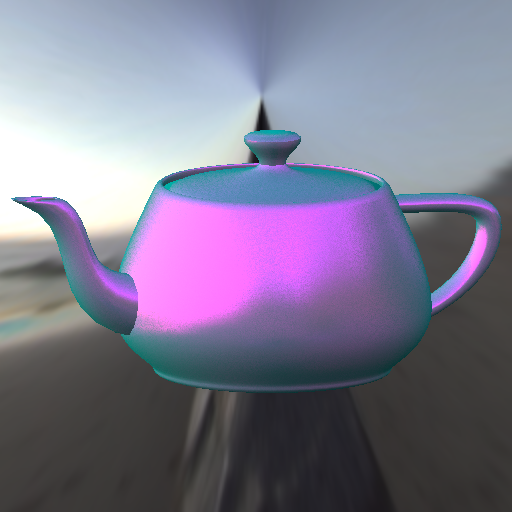
\includegraphics[width=\linewidth]{./Imagens/brdfs/blinn-phong-teapot.png}
    \legend{ \small (a) \textit{Teapot}}
\endminipage\hfill
\minipage{0.32\textwidth}
  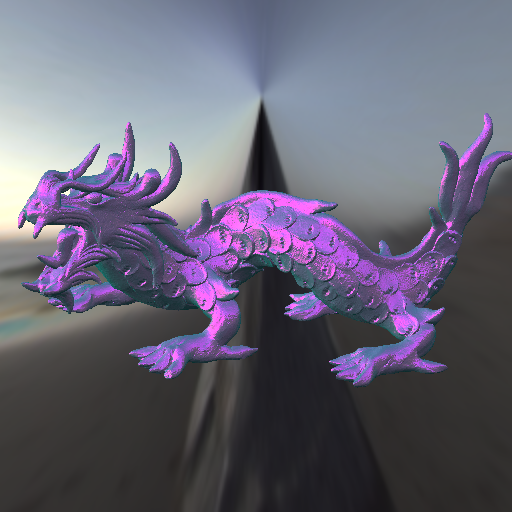
\includegraphics[width=\linewidth]{./Imagens/brdfs/blinn-phong-dragon.png}
    \legend{ \small (b) Dragão de Stanford}
\endminipage\hfill
\minipage{0.32\textwidth}%
  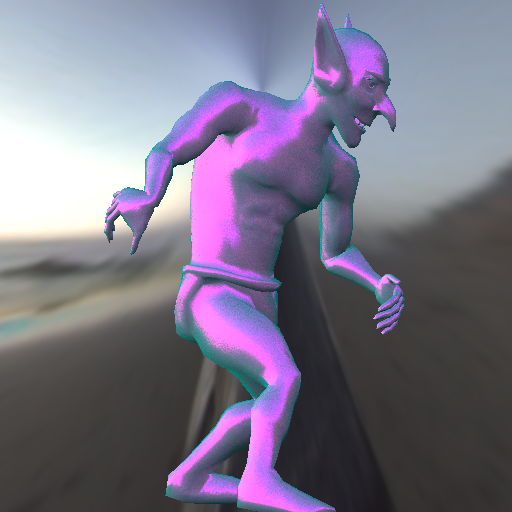
\includegraphics[width=\linewidth]{./Imagens/brdfs/blinn-phong-goblin.png}
    \legend{ \small (c) Goblin}
\endminipage
\end{figure}

